%!TEX root=./pfc.tex
\chapter[Instalación y desinstalación]{\label{}
Instalación y desinstalación}

Como se puede suponer, al existir una filosofía de comunicación cliente-servidor, el sistema deberá contar con al menos dos equipos, uno que haga las veces de cliente y el otro de servidor. Sin embargo, esto no quiere decir que puedan estar involucrados más equipos. Es más, el sistema está diseñado de tal manera que varios clientes, cada uno con su equipo, puedan acceder al servicio del servidor en cualquier momento y desde cualquier lugar. De esta manera, la instalación y configuración de cada equipo dependerá de para qué se utilice.

En la parte del cliente este apartado es muy simple, pues lo único que se necesita es un ordenador con conexión a internet y un navegador Web, como puede ser Mozilla Firefox, Internet Explorer, Google Chrome, Safari...

Sin embargo, la parte servidor necesitará de una instalación de programas y de una configuración del sistema mucho más específica y compleja.

En el siguiente apartado, se explicarán todos los pasos a realizar para una correcta instalación y configuración de la parte servidor del sistema (\emph{mod-wikicode}).

\section{Instalación y configuración de \emph{mod-wikicode}}

El sistema \emph{mod-wikicode} necesitará la instalación de los siguientes programas:

\begin{description}
	
	\item[Moodle:] Sistema de gestión de cursos de libre distribución que ayuda a crear comunidades de aprendizaje en línea. Todas las versiones pueden encontrarse gratuitamente en \emph{http://www.moodle.org}. Aproximadamente se necesitarán unos 38 Mb de disco duro.
	
	\item[JQuery:] Biblioteca open-source de JavaScript que permite simplificar la manera de interactuar con los documentos HTML, manipular el árbol DOM, manejar eventos, desarrollar animaciones y agregar interacción con la técnica AJAX a páginas web. Se puede descargar desde \emph{http://jquery.com/} y su tamaño es únicamente de 32 Kb.
	
	\item[Servidor HTTP Apache:] Servidor web HTTP multiplataforma con licencia de Software Libre. Podemos acceder a su contenido desde \emph{http://httpd.apache.org/}.
	
	\item[MySQL:] Sistema de gestión de bases de datos relacional, multihilo y multiusuario. Dispone de licencia GPL y podemos acceder a él desde su página oficial \emph{http://www.mysql.com/}.
	
	\item[PHP:] Intérprete para los lenguajes script Perl y PHP. Hay varias versiones estables y podemos descargarlo desde su Web Oficial \emph{http://www.php.net/}.
	
	\item[GCC:] Conjunto de compiladores creados por el proyecto GNU. GCC es software libre y lo distribuye la FSF bajo la licencia GPL. Disponible en su web oficial \emph{http://gcc.gnu.org/}.
	
	\item[MinGW:] Opcional. Implementación de los compiladores GCC para la plataforma Win32, que permite migrar la capacidad de este compilador en entornos Windows. MinGW incluye un conjunto de la API de Win32, permitiendo un desarrollo de aplicaciones nativas para esa plataforma, pudiendo generar ejecutables y bibliotecas usando la API de Windows. Descargable desde \emph{http://www.mingw.org/}.
	
\end{description}

\subsection{Instalación de Moodle (Microsoft Windows)}

Para facilitar la instalación bajo este sistema operativo nos apoyaremos en el sistema de infraestructura de Internet definido por el acrónimo WAMP, el cual es un conjunto de aplicaciones necesarios para montar un servidor para Windows. El acrónimo se refiere a \textbf{W}indows, \textbf{A}pache, \textbf{M}ySQL y \textbf{P}HP. Uno de los más populares es \emph{WampServer}, el cual podemos descargar desde \emph{http://www.wampserver.com/en/}.

Una vez tengamos descargado este sistema, procederemos también a la descarga del anteriormente descrito \emph{MinGW}. Este será el compilador que usemos bajo Windows.

Los pasos para la instalación del sistema bajo este sistema operativo se enumeran a continuación:

\begin{enumerate}
	\item Descargar e instalar WampServer con las opciones por defecto.
	\item Descargamos y ejecutamos la última versión del instalador de MinGW de su página web oficial. Posteriormente seleccionamos el directorio sobre el que queremos instalar MinGW, donde se aconseja no utilizar espacios en blanco para comodidad posterior. Por último seleccionamos los componentes opcionales que queramos instalar. Por defecto no es necesario ningún componente adicional, pero podemos instalar aquellas librerías que deseemos en función del código que deseemos implementar.
	\item Si bien no es necesario añadir a la variable de entorno \emph{PATH} la ruta donde hayamos instalado nuestro compilador, es aconsejable.
	\item El siguiente paso es instalar Moodle. Para ello debemos descargar el paquete desde su web oficial y descomprimirlo en nuestro directorio www de Apache. Este directorio se encontrará en la ruta que hayamos instalado Wamp.
\end{enumerate}

\subsection{Instalación de Moodle (Mac OS)}

Para facilitar la instalación bajo este sistema operativo nos apoyaremos en el sistema de infraestructura de Internet definido por el acrónimo MAMP, el cual es un conjunto de aplicaciones necesarios para montar un servidor para Mac OS. El acrónimo se refiere a \textbf{M}acintosh, \textbf{A}pache, \textbf{M}ySQL y \textbf{P}HP. Uno de los más populares es \emph{Mamp Pro}, el cual podemos descargar desde \emph{http://www.mamp.info/}.

Para instalar GCC (recomendable) los pasos son los siguientes:

\begin{enumerate}
	\item Descargamos el paquete XCode desde \textbf{http://connect.apple.com/}. Es necesario registrar una cuenta de Apple Developer Connection.
	\item Una vez estemos registrados, nos logueamos y hacemos click en \textbf{Download Software} y posteriormente en \textbf{Developer Tools}. Buscamos el link a \textbf{Xcode Tools (version) – CD Image} y hacemos click sobre él.
	\item Ejecutamos el paquete descargado, haciendo doble click sobre él, y seleccionamos GCC para instalarlo.
\end{enumerate} 
	
Opcionalmente también podemos instalar MinGW bajo este sistema operativo. Esto nos da la posibilidad de hacer Cross Compiling, lo que nos permite desde Mac OS compilar aplicaciones para Windows. Si deseamos instalar MinGW (recomendable) los pasos son estos:

\begin{enumerate}
	\item Descargamos el paquete desde la web \emph{http://crossgcc.rts-software.org/doku.php}.
	\item Ejecutamos el paquete descargado, el cual se descomprime en el directorio \emph{/usr/local/i386-mingw32-3.4.5} por ejemplo para esta versión de MinGW.
\end{enumerate}

Por lo tanto, los pasos a seguir son los siguientes:

\begin{enumerate}
	\item Descargar e instalar MAMP Pro con las opciones por defecto.
	\item Descargamos e instalamos GCC y/o MinGW siguiendo los pasos explicados anteriormente.
	\item Si bien no es necesario añadir a la variable de entorno \emph{PATH} la/s ruta/s donde hayamos instalado nuestro/s compilador/es, es aconsejable.
	\item El siguiente paso es instalar Moodle. Para ello debemos descargar el paquete desde su web oficial y descomprimirlo en nuestro directorio www de Apache. Este directorio se encontrará en la ruta que hayamos instalado Mamp.
\end{enumerate}

\subsection{Instalación de Moodle (GNU/Linux)}

Para facilitar la instalación bajo este sistema operativo nos apoyaremos en el sistema de infraestructura de Internet definido por el acrónimo LAMP, el cual es un conjunto de aplicaciones necesarios para montar un servidor para Linux. El acrónimo se refiere a \textbf{L}inux, \textbf{A}pache, \textbf{M}ySQL y \textbf{P}HP. Uno de los más populares es \emph{Lamp Server}, el cual podemos descargar desde el sistema de gestión de paquetes de nuestra distribución.

Opcionalmente también podemos instalar MinGW bajo este sistema operativo. Esto nos da la posibilidad de hacer Cross Compiling, lo que nos permite desde Linux compilar aplicaciones para Windows. Si deseamos instalar MinGW (recomendable) los pasos son estos:
	
\begin{enumerate}
	\item Iniciamos nuestro gestor de paquetes.
	\item Buscamos e instalamos el paquete de nombre mingw32.
\end{enumerate}	
	
\begin{enumerate}
	\item Iniciamos nuestro gestor de paquetes, buscamos e instalamos Lamp Server.
	\item Instalamos MinGW con los pasos descritos anteriormente.
	\item Si bien no es necesario añadir a la variable de entorno \emph{PATH} el directorio bin de donde hayamos instalado mingw32, es aconsejable.
	\item El siguiente paso es instalar Moodle. Para ello debemos descargar el paquete desde su web oficial y descomprimirlo en nuestro directorio www de Apache. Este directorio se encontrará en la ruta \emph{/var/www/}.
\end{enumerate}

\subsection{Puesta en marcha de las distintas aplicaciones}

Otro hecho importante en el que debe hacerse hincapié es la manera en la que se deben poner en marcha las distintas aplicaciones. Realmente sólo nos hará falta con tener una aplicación en ejecución: el servidor Wamp/Mamp/Lamp.

Para ejecutar el servidor bastará con acceder a la aplicación que se nos haya creado tras haberla instalado y pulsar el botón de Iniciar Servidores. La aplicación se encargará ella sola de iniciar los distintos servicios.

\begin{figure}[h]
	\label{wamp.eps}
	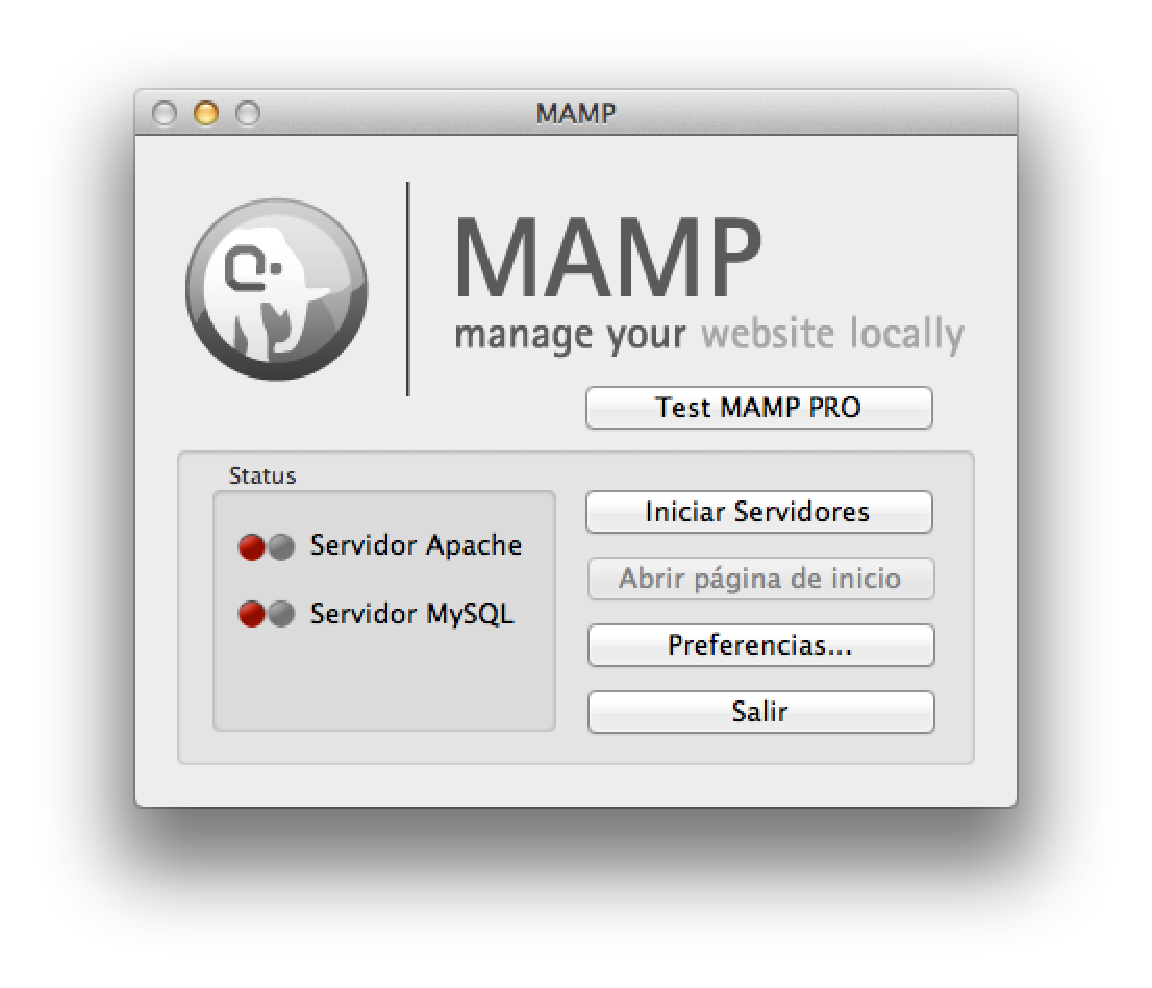
\includegraphics[width=\textwidth]{./img/wamp.eps}
	\caption{MAMP corriendo bajo Mac OS X}
\end{figure}

\subsection{Instalación del módulo \emph{mod-wikicode} en Moodle}

Puesto que el módulo que ha sido desarrollado en este proyecto está disponible tanto para la versión 1.x como para la 2.x de Moodle, a continuación se describe como instalarlo en dichas versiones.

\subsubsection{Instalación en Moodle 1.x}

En nuestro directorio del módulo tendremos las siguientes carpetas:  \emph{./lang} y  \emph{./mod}. Será necesario copiar los archivos en el interior de estos directorios a la ruta de nuestra instalación de nuestra instalación  \emph{Moodle}.

Una vez hayamos copiado estos archivos, haremos login como usuario administrador en Moodle y pulsaremos el botón Notifications:

\vspace{1cm}

\begin{figure}[h]
	\label{Notifications1x.eps}
	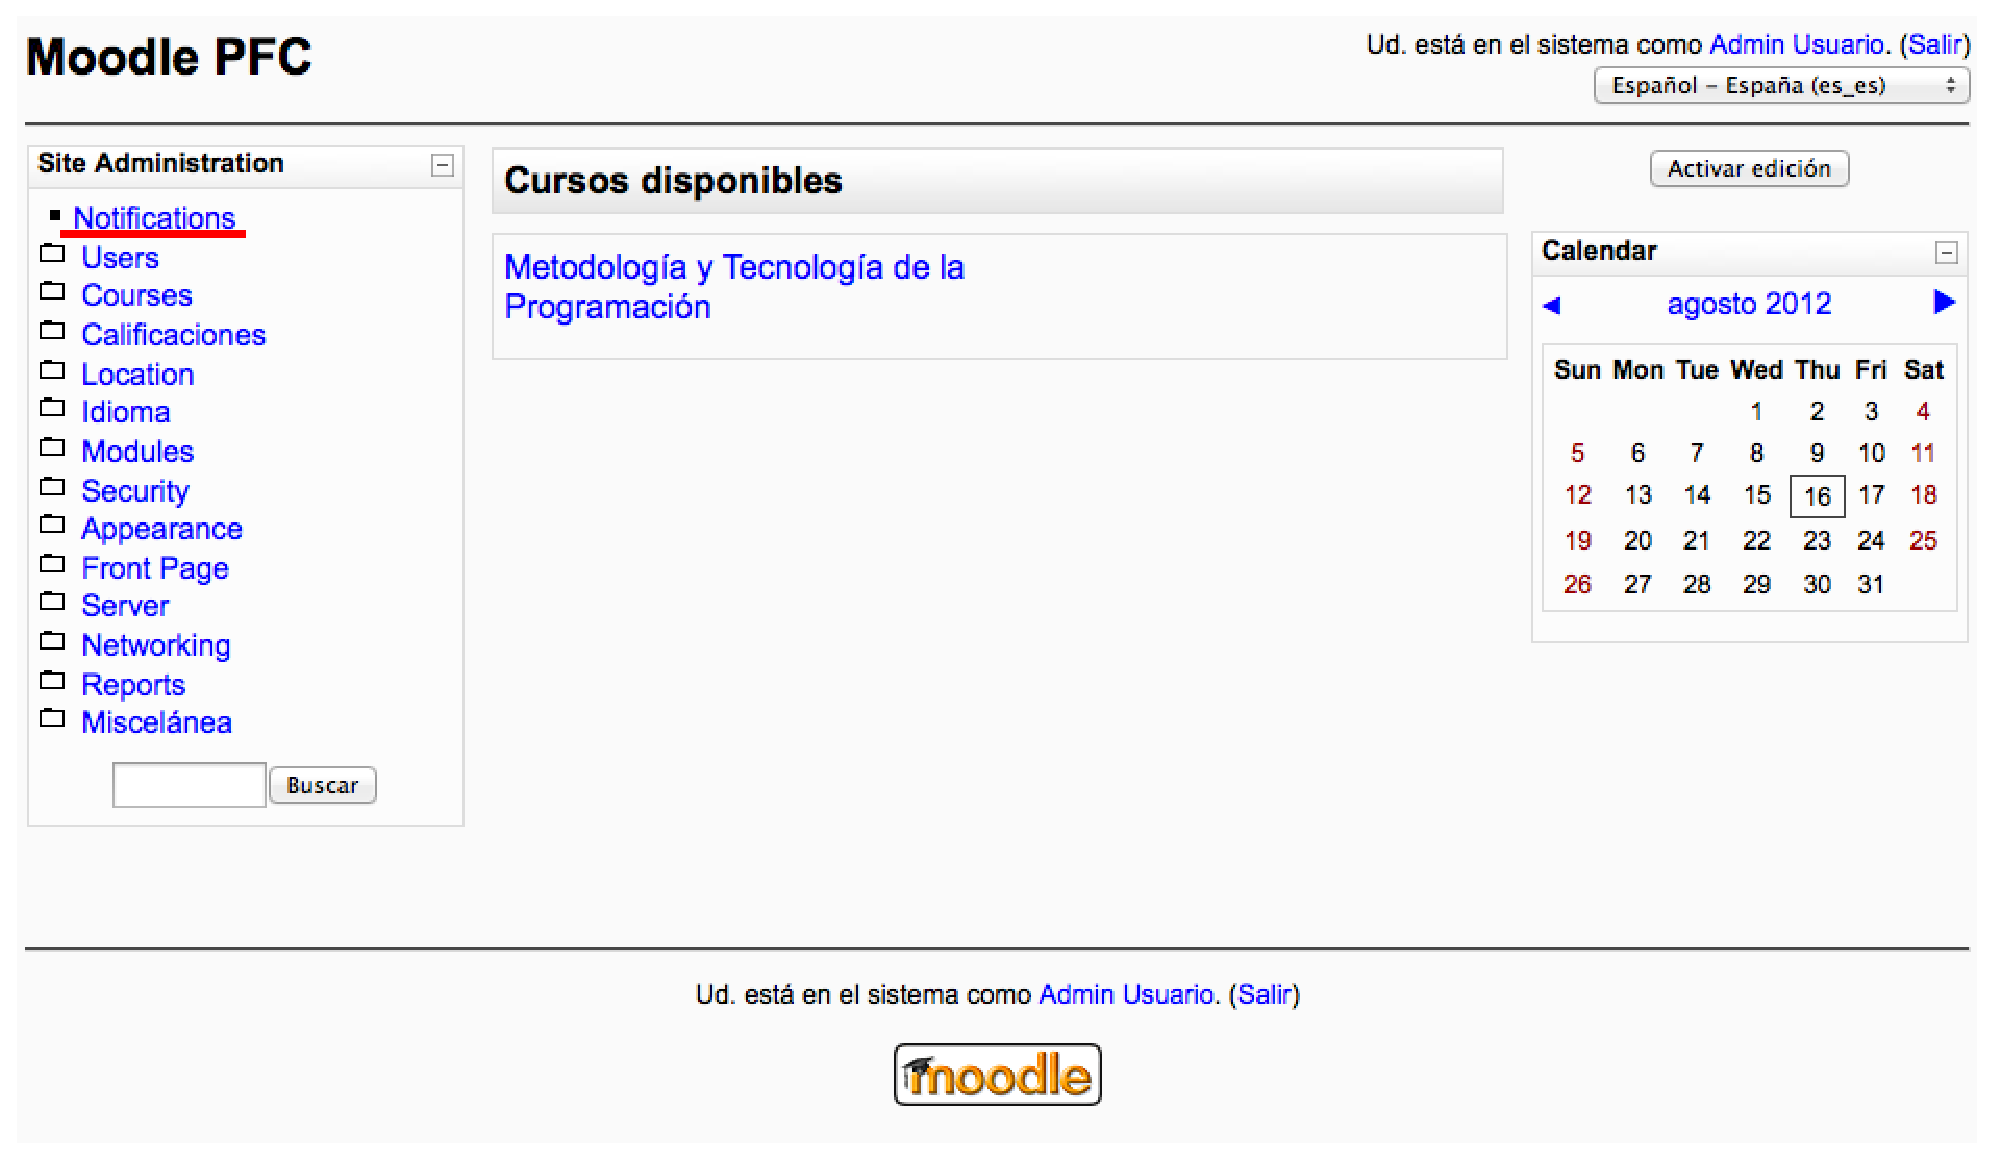
\includegraphics[width=\textwidth]{./img/Notifications1x.eps}
	\caption{Pantalla principal del administrador en Moodle 1.x}
\end{figure}

El sistema Moodle se encargará a partir de ese momento automáticamente de todo y el módulo quedará funcionalmente instalado.

\subsubsection{Instalación en Moodle 2.x}

En nuestro directorio del módulo tendremos únicamente una carpeta denominada \emph{/mod} y en su interior otra con el nombre \emph{/wikicode}. Simplemente tendremos que copiar esta última carpeta al directorio \emph{/mod} original de nuestro sistema Moodle. Una vez hayamos hecho esta copia bastará con hacer login como admin y todo se instalará automáticamente tras hacer las comprobaciones oportunas.

\begin{figure}[h]
	\label{installwikicode2x.eps}
	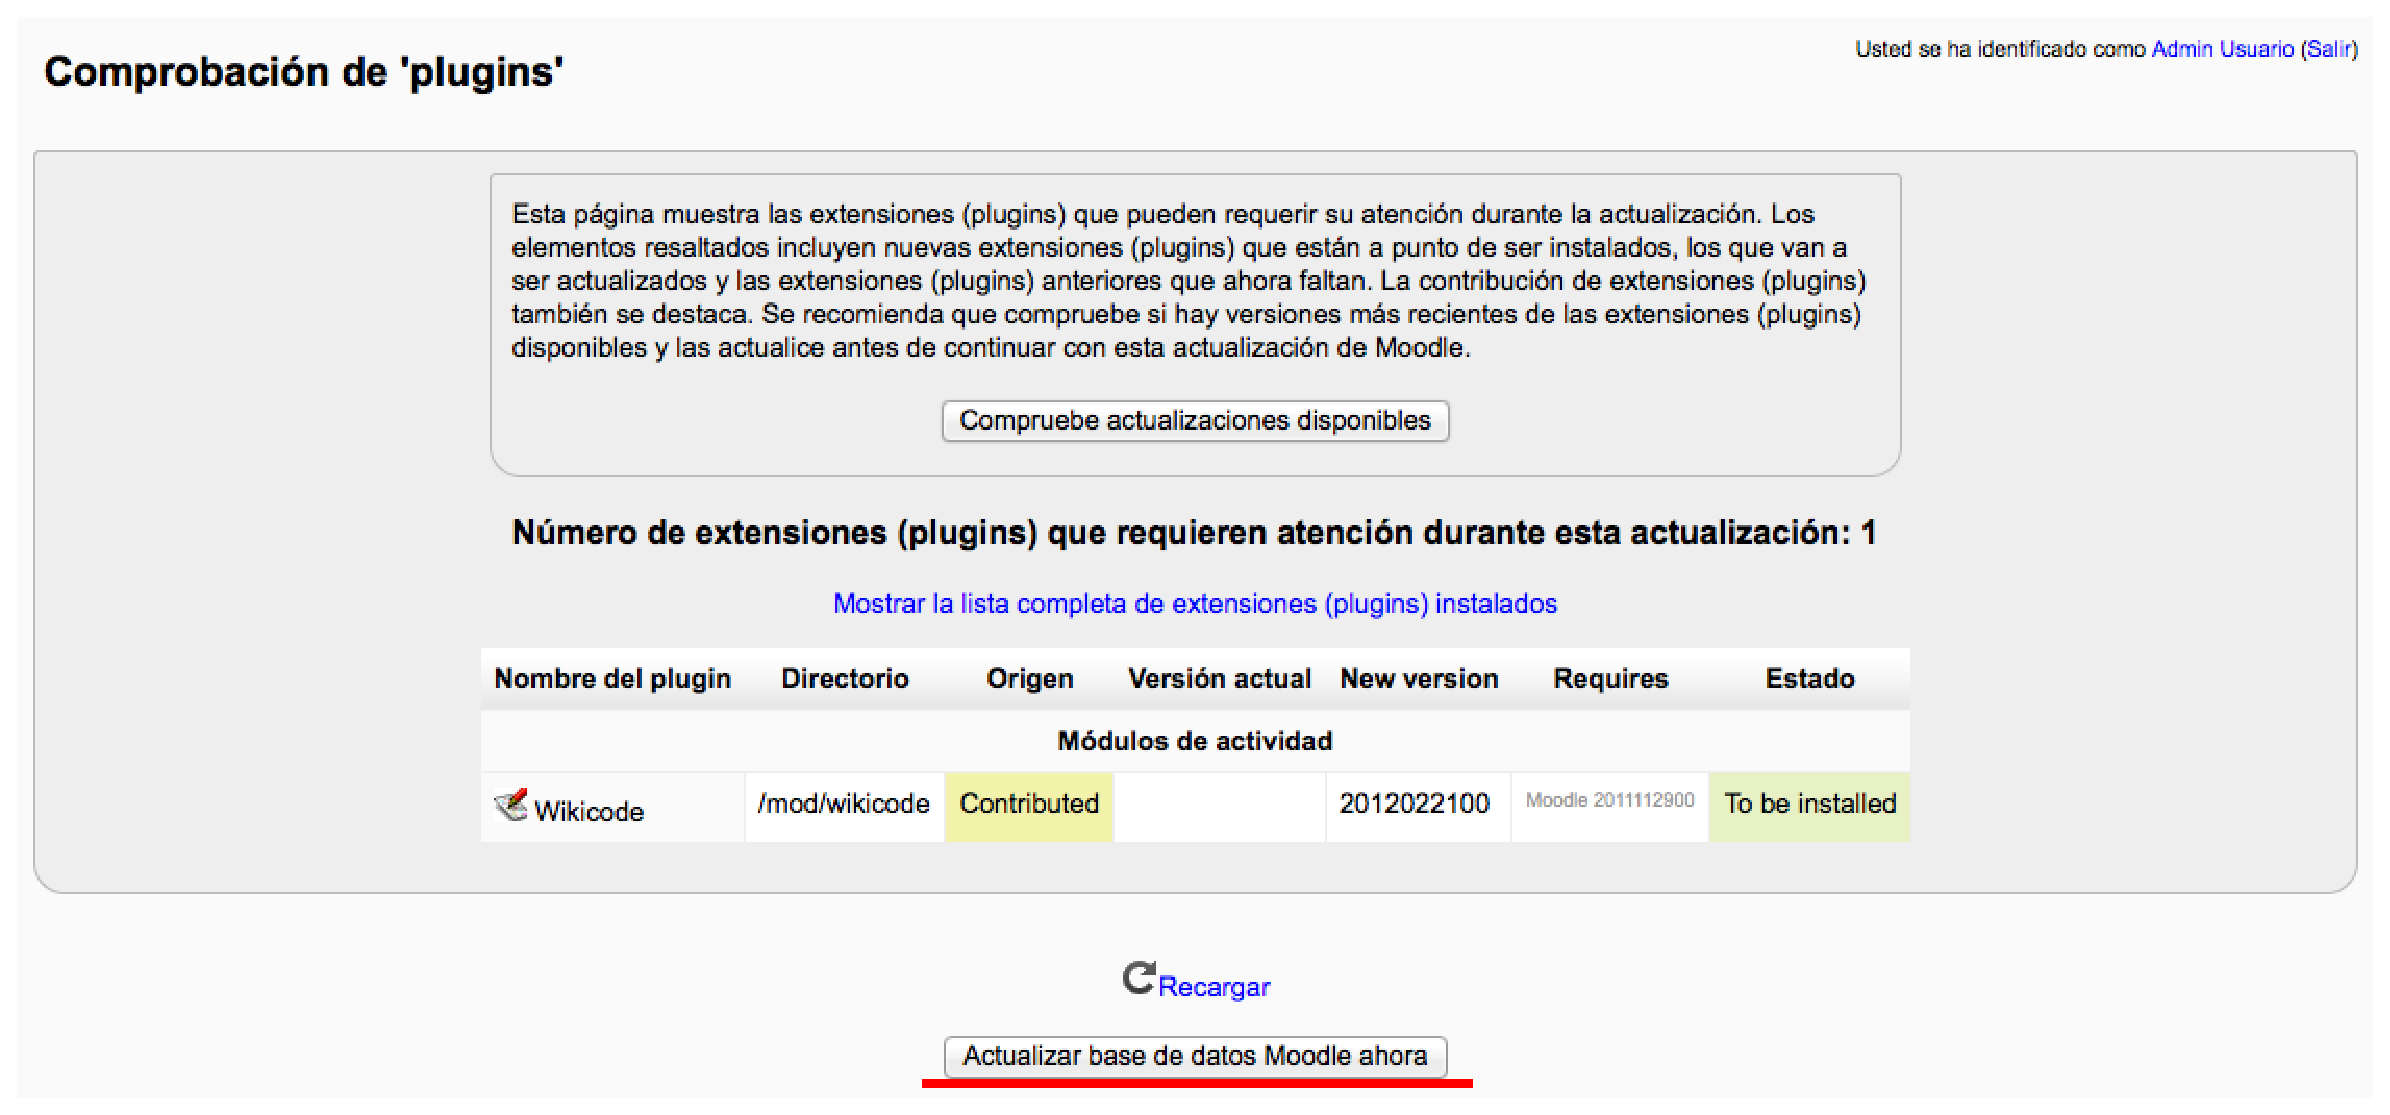
\includegraphics[width=\textwidth]{./img/installwikicode2x.eps}
	\caption{Instalación del módulo Wikicode en Moodle 2.x}
\end{figure}

\subsection{Actualización de JQuery}

Dentro de nuestro módulo, en el directorio \emph{/mod/wikicode/js}, tendremos un archivo denominado \textbf{jquery.js}. Esta archivo contiene la versión de \emph{JQuery 1.8.0}. Con esta versión todo funciona de modo correcto, pero si se quisiera actualizar con una versión futura para mejorar el rendimiento o añadir una nueva funcionalidad bastaría con actualizar dicho fichero.

\section{Desinstalación}

La desinstalación se trata de un proceso muy sencillo en nuestro caso. Puesto que tanto Moodle como el módulo funcionan con un intérprete, bastara con desinstalar nuestro conjunto de aplicaciones *AMP.

\subsection{Desinstalación en Windows. WampServer y MinGW.}
En primer lugar eliminaremos el servidor WAMP. Esta aplicación la podemos eliminar de dos maneras bastante simples: La primera es accediendo al Panel de Control, desde ahí seleccionamos \emph{"Agregar o Quitar Programas"} y lo marcamos para su correcta desinstalación. Un modo aún más sencillo es desde un terminal de Windows ejecutar el siguiente comando:

\begin{lstlisting}[style=consola]
	C:\Wamp\unins000.exe
\end{lstlisting}

Para desinstalar MinGW lo podemos hacer también desde la opción correspondiente dentro de \emph{"Agregar o Quitar Programas"}.
	
\subsection{Desinstalación en Mac OS. MAMP. }
Su desinstalación será bastante simple. Nos bastará con arrastrar la carpeta creada en el directorio Aplicaciones a la Papelera del sistema. Tras vaciar la Papelera se habrá eliminado la aplicación por completo.
	
\subsection{Desinstalación en GNU/Linux. Lamp Server y MinGW.}
Desde el propio Gestor de Paquetes que hayamos utilizado para instalar las aplicaciones, buscamos de nuevo la aplicación y la marcamos para desinstalar. Confiramos la operación y el Sistema de Gestión de Paquetes se encargará de borrar todos los archivos.
	
	
	
	
	
	
	
	
	
	
	
	
	
	
	
	
	
	
	
	
	
	
	
	
	
	
	
	